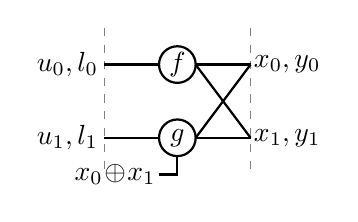
\begin{tikzpicture}[scale=.93, thick]

  \draw[very thin,gray,dashed] (1,.5) -- (1,-1.5);
  \draw[very thin,gray,dashed] (3,.5) -- (3,-1.5);

  %\node at (-.5,1) {layer};
  %\node at (1,.75) {0};
  %\node at (3,.75) {1};

  \node at (.5,0) {$u_0,l_0$};
  \node at (.5,-1) {$u_1,l_1$};

  \draw (1,0) -- (1.75,0);
  \draw (2.25,0) -- (3,0);
  \draw (1,-1) -- (1.75,-1);
  \draw (2.25,-1) -- (3,-1);

  \draw (2,0) circle [radius=.25] node {$f$};
  \draw (2,-1) circle [radius=.25] node {$g$};
  
  \draw (3,-1) -- (2.25,0);
  \draw (3,0) -- (2.25,-1);
  
  \draw (1.75,-1.5) -- ++(.25,0) -- ++(0,.25);
  
  \node at (1.15,-1.5) {$x_0 \!\oplus\! x_1$};

  \node at (3.5,0) {$x_0,y_0$};
  \node at (3.5,-1) {$x_1,y_1$};

\end{tikzpicture}